\section{More Examples of Hypothesis Testing}
%%%%%%%%%%%%%%%%%%%%%%%%%%%%%%%%%%%%%%%%
\begin{frame}
  \frametitle{More Examples}
  Re-do all the CI examples \emph{except} those for proportions as tests. 
\end{frame}
%%%%%%%%%%%%%%%%%%%%%%%%%%%%%%%%%%%%%%%%
\begin{frame}
\begin{block}{Last Time}
Simple Example of Hypothesis Testing: the Pepsi Challenge
\end{block}

\begin{block}{Today and Next Two Lectures}
Hypothesis Testing More Generally
\end{block}

\end{frame}
%%%%%%%%%%%%%%%%%%%%%%%%%%%%%%%%%%%%%%%%

\begin{frame}
\frametitle{Hypothesis: Assertion about Population(s)}
	\begin{itemize}
	\item A Big Mac contains, on average, 550 kcal: \alert{$\mu = 550$}
	\item Midterm 2 was harder than Midterm 1: \alert{$\mu_{1} >\mu_2$}
	\item Equal proportions of Republicans and Democrats know that John Roberts is the chief justice of SCOTUS: \alert{$p = q$}
	\item Google stock is riskier than IBM stock: \alert{$\sigma^2_{X} > \sigma^2_{Y}$}
	\item There is no correlation between height and income: \alert{$\rho = 0$} 
	\end{itemize}
\end{frame}

%%%%%%%%%%%%%%%%%%%%%%%%%%%%%%%%%%%%%%%%
\begin{frame}
	\frametitle{Hypothesis Testing: Try to 
	Find Evidence \emph{Against} $H_0$}
\begin{block}
	{Null Hypothesis: $H_0$}
	\begin{itemize}
		\item Start off assuming $H_0$ is true --
		 ``innocent until proven guilty''
		\item ``Under the Null'' = Assuming the null is true
		\item $H_0$ $\Rightarrow$ know something about population, can calculate probs.
	\end{itemize}
\end{block}
\begin{alertblock}
	{This Course: \emph{Simple} Null Hypotheses}
	$H_0\colon f(\mbox{Parameters}) = \mbox{Known Constant}$, for example
	\begin{itemize}
		\item $\mu_1 - \mu_2 = 0$
		\item $p = 0.5$
		\item $\mu = 0$
		\item $\sigma^2_X/\sigma^2_Y = 1$
	\end{itemize}
\end{alertblock}
\end{frame}
%%%%%%%%%%%%%%%%%%%%%%%%%%%%%%%%%%%%%%%%
\begin{frame}
	\frametitle{How do I know what my null hypothesis is?}
	There is no rule I can give you for this: it depends on the problem. Here are some guidelines:
	\begin{itemize}
		\item It will take the form $f(\mbox{Parameters}) = \mbox{Known Constant}$
		\item Nulls are typically things like ``there is no effect,'' ``these two groups are not different,'' i.e.\ the \emph{status quo}. 
		\item Nulls are \emph{very specific}: we need to be able to do probability calculations under the null -- c.f.\ the Pepsi Challenge.
	\end{itemize}
\end{frame}
%%%%%%%%%%%%%%%%%%%%%%%%%%%%%%%%%%%%%%%%
\begin{frame}[t]
	\frametitle{Example: How many calories in a Big Mac? \hfill 
\includegraphics[scale = 0.05]{./images/clicker}}
\begin{itemize}
	\item According to McDonald's: 550 kcal on average
	\item Measure calories in random sample of $9$ Big Macs: $X_1, \hdots, X_{9} \sim \mbox{iid } N(\mu, \sigma^2)$
\end{itemize}

\vspace{1em}

\alert{If we wanted to test McDonald's claim, what would be $H_0$?}
\begin{enumerate}[(a)]
	\item $\sigma^2 = 1$
	\item $\mu = 0$
	\item $\mu > 550$ 
	\item $\mu = 550$
	\item $\mu \neq 550$
\end{enumerate}
\end{frame}
%%%%%%%%%%%%%%%%%%%%%%%%%%%%%%%%%%%%%%%%
\begin{frame}[t]
	\frametitle{Example: How many calories in a Big Mac? \hfill 
\includegraphics[scale = 0.05]{./images/clicker}}
\begin{itemize}
	\item According to McDonald's: 550 kcal on average
	\item Measure calories in random sample of $9$ Big Macs: $X_1, \hdots, X_{9} \sim \mbox{iid } N(\mu, \sigma^2)$
\end{itemize}

\vspace{1em}

\alert{If McDonald's is telling the truth, approximately what value should we get for the sample mean caloric content of the $9$ Big Macs?} 
\end{frame}
%%%%%%%%%%%%%%%%%%%%%%%%%%%%%%%%%%%%%%%%
\begin{frame}[t]
	\frametitle{Example: How many calories in a Big Mac? \hfill 
\includegraphics[scale = 0.05]{./images/clicker}}
\begin{itemize}
	\item According to McDonald's: 550 kcal on average
	\item Measure calories in random sample of $9$ Big Macs: $X_1, \hdots, X_{9} \sim \mbox{iid } N(\mu, \sigma^2)$
\end{itemize}

\vspace{1em}

\alert{If the sample mean does not equal 550, does this prove that McDonald's is lying?}
\begin{enumerate}[(a)]
	\item Yes
	\item No
	\item Not Sure
\end{enumerate}
\end{frame}
%%%%%%%%%%%%%%%%%%%%%%%%%%%%%%%%%%%%%%%%
\begin{frame}
	\frametitle{How to find evidence against $H_0$? Test Statistic!}
	\begin{block}
		{Test Statistic: $T_n$}
		A statistic that gives us information about the parameter we are testing and has a \emph{known} sampling distribution \emph{under $H_0$}.
	\end{block}
\end{frame}
%%%%%%%%%%%%%%%%%%%%%%%%%%%%%%%%%%%%%%%%
%\begin{frame}[t]
%	\frametitle{Example: How many calories in a Big Mac? \hfill 
\includegraphics[scale = 0.05]{./images/clicker}}
%\begin{itemize}
%	\item Measure calories in random sample of $n$ Big Macs: $X_1, \hdots, X_9 \sim \mbox{iid } N(\mu, \sigma^2)$
%	\item $H_0\colon \mu = 550$
%\end{itemize}
%
%\vspace{1em}
%
%\alert{Which of these should we use as our test statistic?}
%\begin{enumerate}[(a)]
%	\item $S^2$
%	\item $\bar{X} - 550$
%	\item $\bar{X}$
%	\item $\bar{X} / S$ 
%	\item $(\bar{X} - 550)/(S/3)$
%\end{enumerate}
%\end{frame}
%%%%%%%%%%%%%%%%%%%%%%%%%%%%%%%%%%%%%%%%
\begin{frame}[t]
	\frametitle{Example: How many calories in a Big Mac? \hfill 
\includegraphics[scale = 0.05]{./images/clicker}}
\begin{itemize}
	\item Measure calories in random sample of $n$ Big Macs: $X_1, \hdots, X_9 \sim \mbox{iid } N (\mu, \sigma^2)$
	\item $H_0\colon \mu = 550$
\end{itemize}

\vspace{1em}

\alert{If McDonald's is telling the truth, i.e.\ under the null, what is \emph{exact}  sampling distribution of $(\bar{X} - 550)/(S/3)$?}
\begin{enumerate}[(a)]
	\item $\chi^2_{9}$
	\item $N(550, 1)$
	\item $F(9, 1)$
	\item $N(0,1)$ 
	\item $t_{8}$
\end{enumerate}
\end{frame}
%%%%%%%%%%%%%%%%%%%%%%%%%%%%%%%%%%%%%%%%
\begin{frame}
	\frametitle{What if the null is false?}

	\begin{block}
		{Alternative hypothesis: $H_1$}
		The \emph{negation} of the null hypothesis.
	\end{block}
	\begin{block}
		{Examples:}
		\begin{enumerate}
			\item 
				\begin{itemize}
					\item $H_0\colon$ This parameter equals 5.
				\item $H_1\colon$ This parameter does \emph{not} equal 5.
		\end{itemize}
			\item 
				\begin{itemize}
					\item $H_0\colon$ There is no difference between these two groups.
					\item $H_1\colon$ There \emph{is} a difference between these two groups.
				\end{itemize}
		\end{enumerate}
		
	\end{block}

	\alert{Sometimes we only care about \emph{certain kinds} of violations of $H_0$...}
\end{frame}
%%%%%%%%%%%%%%%%%%%%%%%%%%%%%%%%%%%%%%%%
\begin{frame}
\frametitle{One-sided vs.\ Two-sided Alternative}
\alert{Let $\theta$ be a population parameter and $\theta_0$ be a specified constant.}
\begin{block}
	{Null Hypothesis}
\begin{itemize}
	\item $H_0\colon \theta = \theta_0$
\end{itemize}\end{block}
	\begin{block}{Two-sided Alternative}
		\begin{itemize}
			\item $H_1\colon \theta \neq \theta_0$
		\end{itemize}
\end{block}
	\begin{block}{One-sided Alternative}
		Two possibilities, depending on the problem at hand:
		\begin{itemize}
			\item $H_1\colon \theta > \theta_0$
			\item $H_1\colon \theta < \theta_0$
		\end{itemize}
\end{block}
\end{frame}

%%%%%%%%%%%%%%%%%%%%%%%%%%%%%%%%%%%%%%%%
\begin{frame}
\frametitle{Example: Suing McDonald's \hfill 
\includegraphics[scale = 0.05]{./images/clicker}}

A class action lawsuit claims that McDonald's has been  understating the caloric content of the ``Big Mac,'' misleading consumers into thinking the sandwich is healthier than it really is. McDonald's claims the sandwich contains $550$ kcal on average. \\

\vspace{1em}
\alert{Suppose you're the judge in this case. What is your alternative hypothesis?}

	\begin{enumerate}[(a)]
		\item $H_1\colon \mu \neq 550$ kcal
		\item $H_1\colon \mu < 550$ kcal
		\item $H_1\colon \mu > 550$ kcal
		\item $H_1\colon \mu = 550$ kcal
\end{enumerate}
\end{frame}
%%%%%%%%%%%%%%%%%%%%%%%%%%%%%%%%%%%%%%%%

\begin{frame}
\frametitle{Example: Quality Control at McDonald's \hfill 
\includegraphics[scale = 0.05]{./images/clicker}}

You are a senior manager at McDonald's and are concerned that franchises may be deviating from company policy on the calorie count of a Big Mac sandwich, which is supposed to be 550 kcal on average. Because intervening is costly, you will only take action is there is strong evidence of deviation from company policy. \\

\vspace{1em}

\alert{What is your alternative hypothesis?}
	\begin{enumerate}[(a)]
		\item $H_1\colon \mu \neq 550$ kcal
		\item $H_1\colon \mu < 550$ kcal
		\item $H_1\colon \mu > 550$ kcal
		\item $H_1\colon \mu = 550$ kcal
\end{enumerate}
\end{frame}
%%%%%%%%%%%%%%%%%%%%%%%%%%%%%%%%%%%%%%%%%
\begin{frame}
	\frametitle{Decision Rule: When should we reject $H_0$?}
	\begin{itemize}
		\item Test statistic: RV with known sampling distribution under $H_0$
		\item McDonald's Example: $T_n = 3(\bar{X} - 550)/S$
		\item \emph{Random} since $\bar{X}$ and $S$ are RVs under random sampling: functions of $X_1, \hdots, X_9$.
		\item Observed dataset: \emph{realizations} $x_1, \hdots, x_9$ of RVs $X_1, \hdots, X_9$
		\item Plug in observed data to get estimates (constants) $\bar{x}$ and $s$.
		\item Plug these into the formula for the test statistic to get a \emph{number} -- this is a \emph{realization} of $T_n$ 
		\item Depending on this number, decide whether to reject $H_0$.
	\end{itemize}
\end{frame}
%%%%%%%%%%%%%%%%%%%%%%%%%%%%%%%%%%%%%%%%%
\begin{frame}
\frametitle{What Form Should the Decision Rule Take?}
\begin{columns}
\begin{column}{6cm}
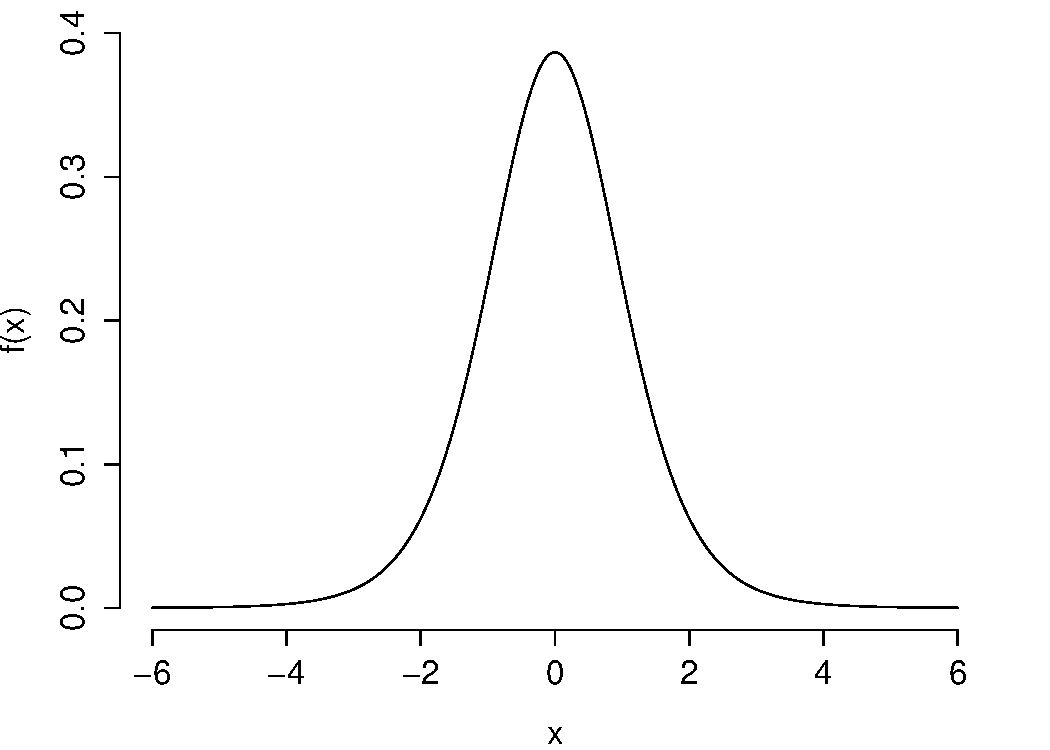
\includegraphics[scale = 0.5]{./images/t_pdf}
\end{column}

\begin{column}{6cm}
$H_0\colon \mu=550 \Rightarrow \displaystyle \frac{\bar{X} - 550}{S/3} \sim t(8)$\\ \pause
\vspace{1em}
One-sided Alternative $H_1\colon \mu > 550$\\ \pause
\vspace{1em}
Two-sided Alternative $H_1\colon \mu \neq 550$ 
\end{column}

\end{columns}
 
\end{frame}
%%%%%%%%%%%%%%%%%%%%%%%%%%%%%%%%%%%%%%%%
\begin{frame}
\frametitle{Example: Suing McDonald's \hfill 
\includegraphics[scale = 0.05]{./images/clicker}}
The plaintiffs allege that McDonald's has \emph{understated} the true caloric content of a Big Mac: it's actually \emph{greater} than 550 kcal. \alert{Suppose the plaintiffs are right. Then what sort of value should we expect the test statistic $3(\bar{X} - 550)/S$ to take on?}

\vspace{1em}
\begin{enumerate}[(a)]
	\item A value \emph{less} than zero.
	\item A value close to zero.
	\item A value \emph{greater} than zero.
\end{enumerate}
\end{frame}
%%%%%%%%%%%%%%%%%%%%%%%%%%%%%%%%%%%%%%%%
\begin{frame}
\frametitle{Example: Quality Control at McDonald's \hfill 
\includegraphics[scale = 0.05]{./images/clicker}}
The senior manager is worried that franchises are deviating from company policy that Big Macs should contain approximately 550 kcal. \alert{If the franchises \emph{are} deviating, what sort of of value should we expect the test statistic $3(\bar{X} - 550)/S$ to take on?}

\vspace{1em}
\begin{enumerate}[(a)]
	\item A value \emph{less} than zero.
	\item A value close to zero.
	\item A value \emph{greater} than zero.
	\item A value different from zero but we can't tell whether it will be positive or negative.
\end{enumerate}
\end{frame}
%%%%%%%%%%%%%%%%%%%%%%%%%%%%%%%%%%%%%%%%
\begin{frame}
\frametitle{What Form Should the Decision Rule Take?}
$X_1, \hdots, X_n \sim \mbox{iid } N(\mu, \sigma^2)$ 
\begin{block}{Common Null Hypothesis $H_0\colon \mu = 550$}
Under $H_0$, $T_n = \sqrt{n}(\bar{X}_n - 550)/S \sim t(n-1)$ 
\end{block}
\begin{block}{One-sided Alternative $H_1\colon \mu > 550$}
Reject $H_0$ if $T_n$ is ``too big'' 
\end{block}
\begin{block}{Two-sided Alternative $H_1\colon \mu \neq 550$} 
Reject $H_0$ if $T_n$ is ``too big'' or ``too small''
\end{block}

\vspace{1em}

\alert{But how big of a discrepancy is ``big enough'' to reject?}
\end{frame}

%%%%%%%%%%%%%%%%%%%%%%%%%%%%%%%%%%%%%%%%
\begin{frame}
	\frametitle{Two Kinds of Mistakes in Hypothesis Testing}
	\begin{block}
		{Type I Error}
		\begin{itemize}
			\item Rejecting the null when it's actually true.
			\item $P(\mbox{Type I Error}) = \alpha\quad \quad$ 
			\alert{$\boxed{\alpha= \mbox{``Significance Level'' of Test}}$}
		\end{itemize}
	\end{block}
	 \begin{block}
		{Type II Error}
		\begin{itemize}
			\item Failing to reject the null when it's false.
			\item $P(\mbox{Type II Error}) = \beta \quad \quad$ 
			\alert{$\boxed{1 - \beta= \mbox{``Power'' of Test}}$}
		\end{itemize}
	\end{block}
	\begin{alertblock}
		{Important!}
		Hypothesis testing \emph{controls} probability of a Type I error since this is assumed to be the \emph{worse} kind of mistake: convicting the innocent.	
	\end{alertblock}
\end{frame}
%%%%%%%%%%%%%%%%%%%%%%%%%%%%%%%%%%%%%%%%%
\begin{frame}
	\frametitle{Construct a Decision Rule to \emph{Fix} $\alpha$ at User-Chosen Level}

	\begin{block}
		{Critical Value $c_{\alpha}$} 
	\begin{itemize}
		\item Threshold for rejecting $H_0$
		\item Chosen so that $P(\mbox{Reject } H_0|H_0 \mbox{ is True}) = \alpha$
		\item Depends on \emph{both} $\alpha$ \emph{and} the alternative hypothesis.
	\end{itemize}
	\end{block}
	\begin{block}
		{One-Sided Alternative}
		Reject $H_0$ if $T_n >$ Critical Value
	\end{block}
	\begin{block}
		{Two-Sided Alternative}
		Reject $H_0$ if $|T_n| >$ Critical Value
	\end{block}
\end{frame}
%%%%%%%%%%%%%%%%%%%%%%%%%%%%%%%%%%%%%%%%%
\begin{frame}
\frametitle{Example: One-sided Alternative $H_1\colon \mu > 550$}
The critical value is chosen to reflect both the alternative hypothesis and the significance level. 
\begin{figure}
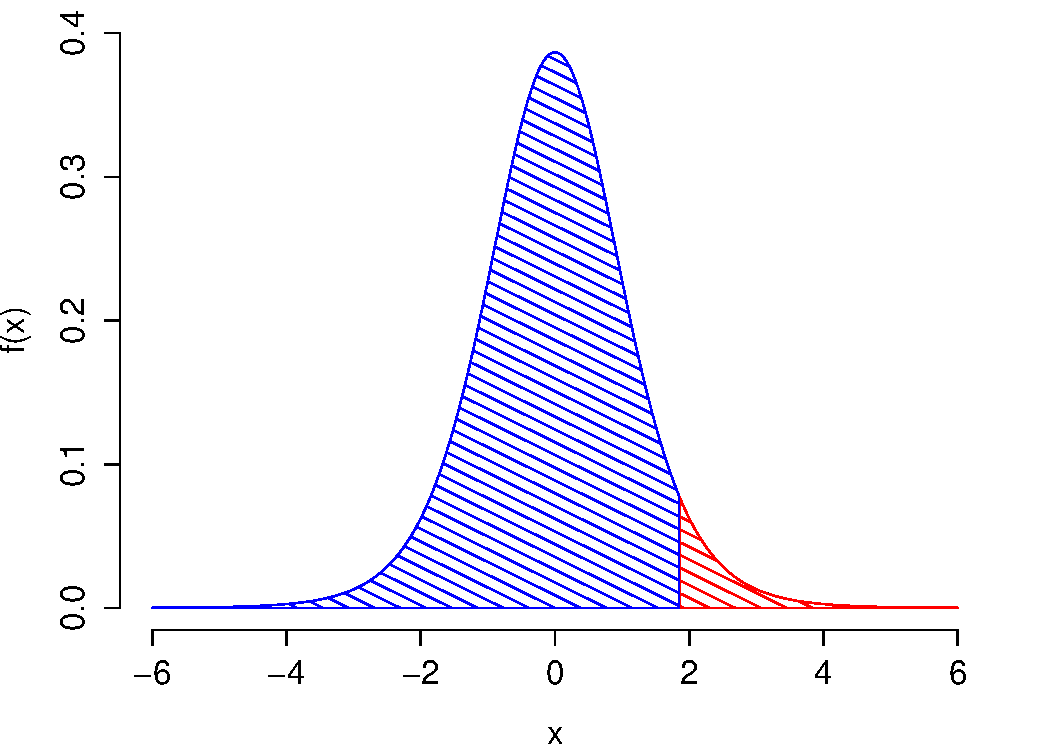
\includegraphics[scale = 0.45]{./images/one_side}
\end{figure}
One-sided Critical Value: \texttt{qt($1-\alpha$, df  = $n-1$)}
\end{frame}


%%%%%%%%%%%%%%%%%%%%%%%%%%%%%%%%%%%%%%%%

\begin{frame}
\frametitle{Example: Two-sided Alternative $H_1\colon \mu \neq 550$}
The critical value is chosen to reflect both the alternative hypothesis and the significance level. 
\begin{figure}
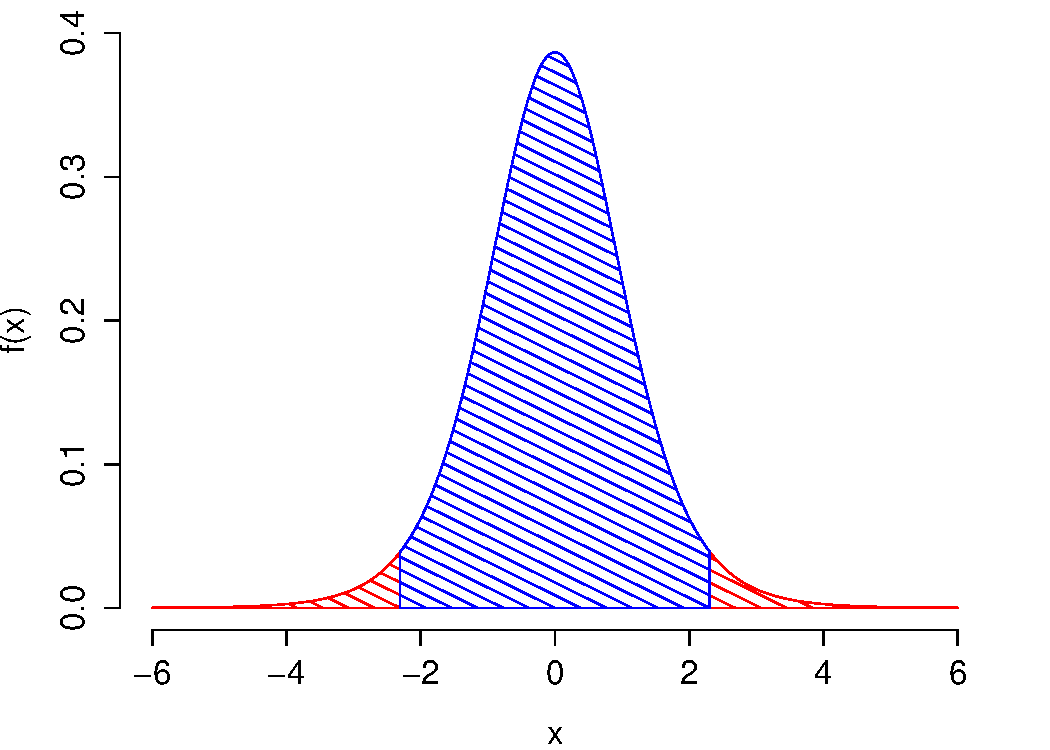
\includegraphics[scale = 0.45]{./images/two_side}
\end{figure}
Two-sided Critical Value: \texttt{qt($1-\alpha/2$, df  = $n-1$)}
\end{frame}

%%%%%%%%%%%%%%%%%%%%%%%%%%%%%%%%%%%%%%%%
\begin{frame}
Suppose, for example, $\alpha = 0.05$, $n = 9$
	\begin{eqnarray*}
		&&\texttt{qt(0.95, df  = 8)}\approx 1.86\\
		 &&\texttt{qt(0.975, df  = 8)}\approx 2.3
	\end{eqnarray*}
\begin{figure}
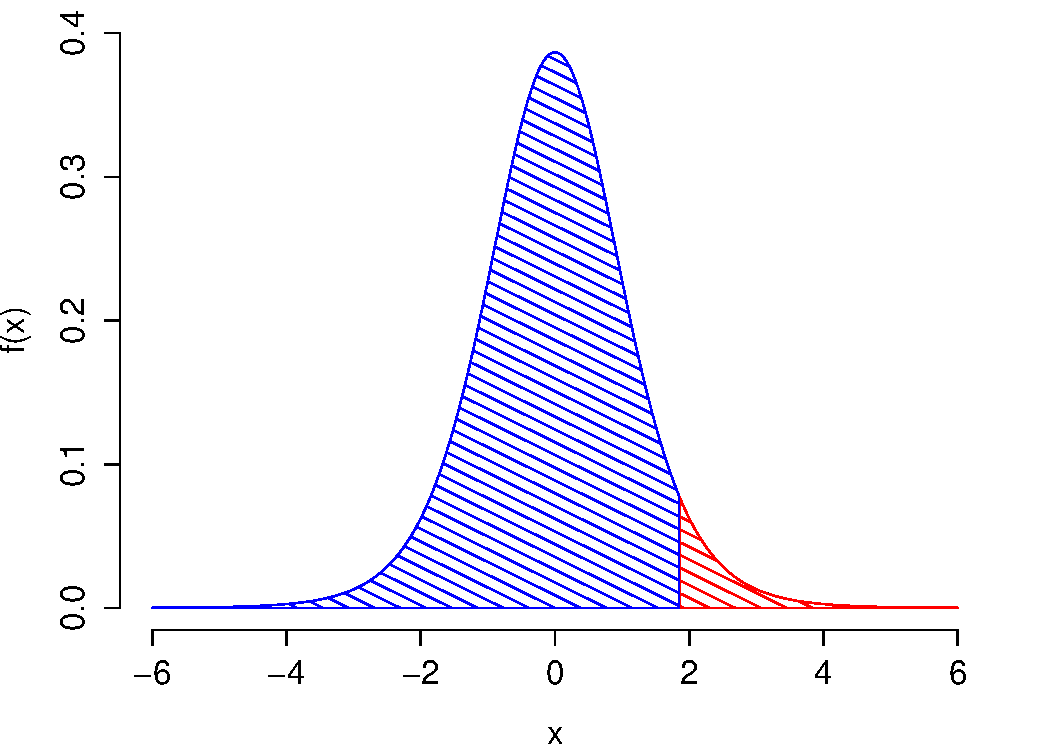
\includegraphics[scale = 0.3]{./images/one_side}
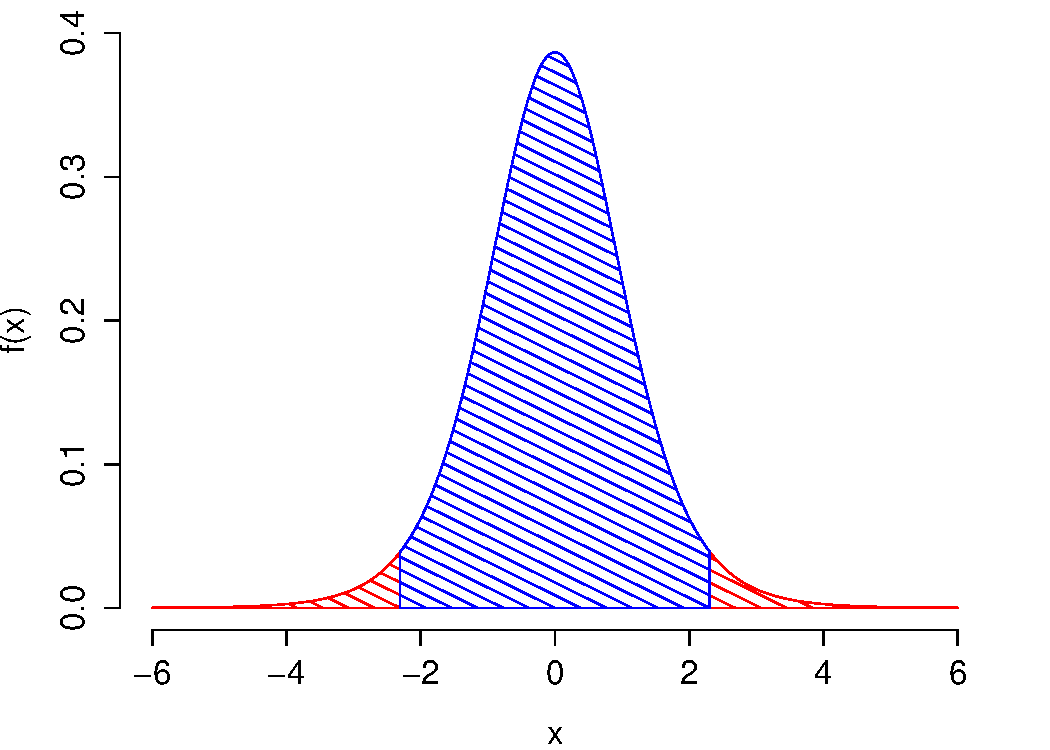
\includegraphics[scale = 0.3]{./images/two_side}
\end{figure}
One-sided Alternative: Reject $H_0$ if $3(\bar{X}_n - 550)/S \geq 1.86$\\
\vspace{0.5em}
Two-sided Alternative: Reject $H_0$ if $\left|3(\bar{X}_n - 550)/S\right| \geq 2.3$\\

\end{frame}

%%%%%%%%%%%%%%%%%%%%%%%%%%%%%%%%%%%%%%%%
\begin{frame}
\frametitle{McDonald's Example\hfill 
\includegraphics[scale = 0.05]{./images/clicker}}
Suppose $n=9$, $\bar{x} = 563$, $s = 34$. What is  the value of our test statistic?

\pause
\vspace{1em}
	$$\frac{563 - 550}{34/\sqrt{9}}= \frac{13}{34/3} \approx 1.14$$


\end{frame}

%%%%%%%%%%%%%%%%%%%%%%%%%%%%%%%%%%%%%%%%
\begin{frame}[t]
\frametitle{McDonald's Example: $\alpha = 0.05$\hfill 
\includegraphics[scale = 0.05]{./images/clicker}}
Recall that:
\begin{eqnarray*}
		&&\texttt{qt(0.95, df  = 8)}\approx 1.86\\
		 &&\texttt{qt(0.975, df  = 8)}\approx 2.3
	\end{eqnarray*}
Based on an observed test statistic of $1.14$, would we reject $H_0$ against the one-sided alternative at the 5\% significance level?
\begin{enumerate}[(a)]
	\item Yes
	\item No
	\item Not Sure
\end{enumerate}

\end{frame}
%%%%%%%%%%%%%%%%%%%%%%%%%%%%%%%%%%%%%%%%
\begin{frame}[t]
\frametitle{McDonald's Example: $\alpha = 0.05$\hfill 
\includegraphics[scale = 0.05]{./images/clicker}}
Recall that:
\begin{eqnarray*}
		&&\texttt{qt(0.95, df  = 8)}\approx 1.86\\
		 &&\texttt{qt(0.975, df  = 8)}\approx 2.3
	\end{eqnarray*}
Based on an observed test statistic of $1.14$, would we reject $H_0$ against the \alert{two-sided} alternative at the 5\% significance level?
\begin{enumerate}[(a)]
	\item Yes
	\item No
	\item Not Sure
\end{enumerate}

\end{frame}

%%%%%%%%%%%%%%%%%%%%%%%%%%%%%%%%%%%%%%%%

\begin{frame}
	\frametitle{Reporting the Results of a Hypothesis Test}
	\begin{block}
		{Lawsuit Example}
		The judge \emph{failed to reject} the null hypothesis that $\mu = 550$ against the one-sided alternative $\mu > 550$ at the 5\% significance level.
	\end{block}
	\begin{block}
		{Quality Control Example}
		The senior manager \emph{failed to reject} the null hypothesis that $\mu =550$ against the two-sided alternative at the 5\% significance level.
	\end{block}
	\begin{block}
		{Interpretation}
		In each of these two cases, there was \emph{insufficient evidence} the initial assumption that $\mu = 550$ \emph{given the significance level used}.
	\end{block}
	\alert{But what if we have used a \emph{different} significance level?}
\end{frame}
%%%%%%%%%%%%%%%%%%%%%%%%%%%%%%%%%%%%%%%%
\begin{frame}
	\frametitle{The P-Value of a Hypothesis Test}
	\begin{block}
		{Two Equivalent Definitions:}
		\begin{enumerate}
			\item Given the value we calculated for our test statistic, what is the \emph{smallest $\alpha$} at which we would have rejected the null?
			\item Under the null, what is the probability of observing a test statistic \emph{at least as extreme} as the one we \emph{actually} observed?
		\end{enumerate}
	\end{block}
	\begin{block}
		{Why Report P-Values?}
		\begin{itemize}
			\item More informative than reporting $\alpha$ and Reject/Fail to Reject
			\item E.g. a p-value of 0.03 means we would have rejected the null for any $\alpha \geq 0.03$ and failed to reject it for any $\alpha < 0.03$ 
		\end{itemize}
	\end{block}
\end{frame}
%%%%%%%%%%%%%%%%%%%%%%%%%%%%%%%%%%%%%%%%

\begin{frame}
\begin{center}
\huge P-Value Depends on Which Alternative We Have Specified!
\end{center}
\end{frame}

%%%%%%%%%%%%%%%%%%%%%%%%%%%%%%%%%%%%%%%%
\begin{frame}
\frametitle{What is the p-value? (One-sided Test)}
\footnotesize
Recall: p-value is \emph{smallest significance level} at which our observed test statistic would cause us to reject $H_0$. \alert{Test statistic is $1.14$. What is the one-sided p-value? }
\begin{figure}
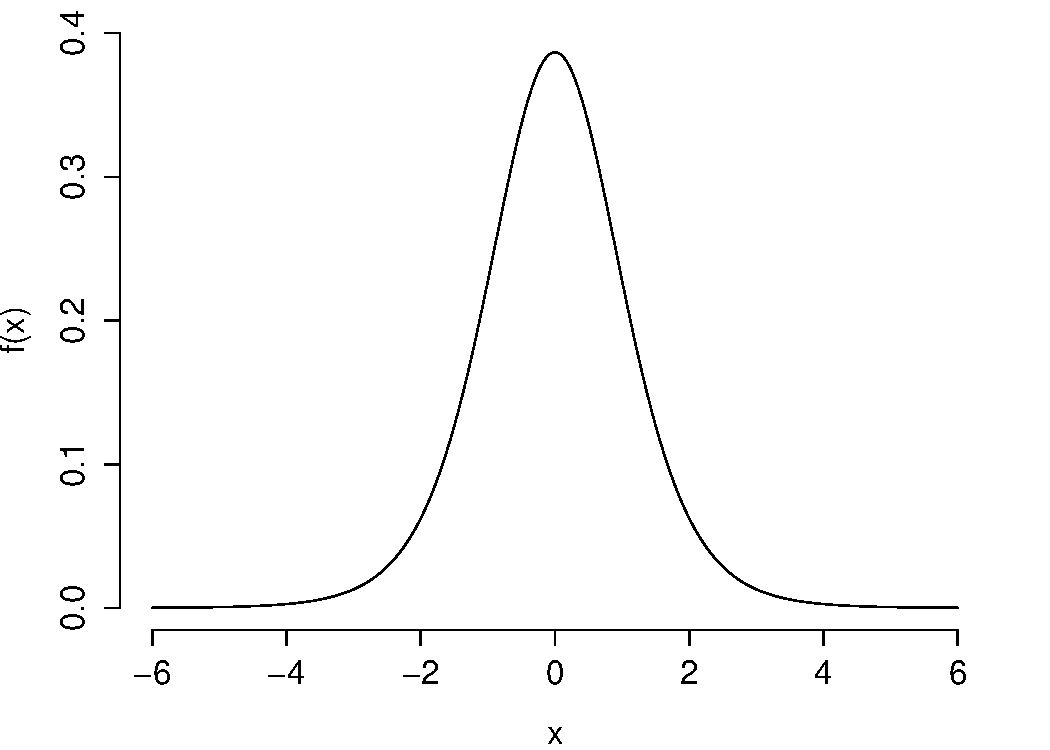
\includegraphics[scale= 0.4]{./images/p_upper1}

\end{figure}

\end{frame}

%%%%%%%%%%%%%%%%%%%%%%%%%%%%%%%%%%%%%%%%
\begin{frame}
\frametitle{What is the p-value? (One-sided Test)}
\footnotesize
Recall: p-value is \emph{smallest significance level} at which our observed test statistic would cause us to reject $H_0$. \alert{Test statistic is $1.14$. What is the one-sided p-value? }
\begin{figure}
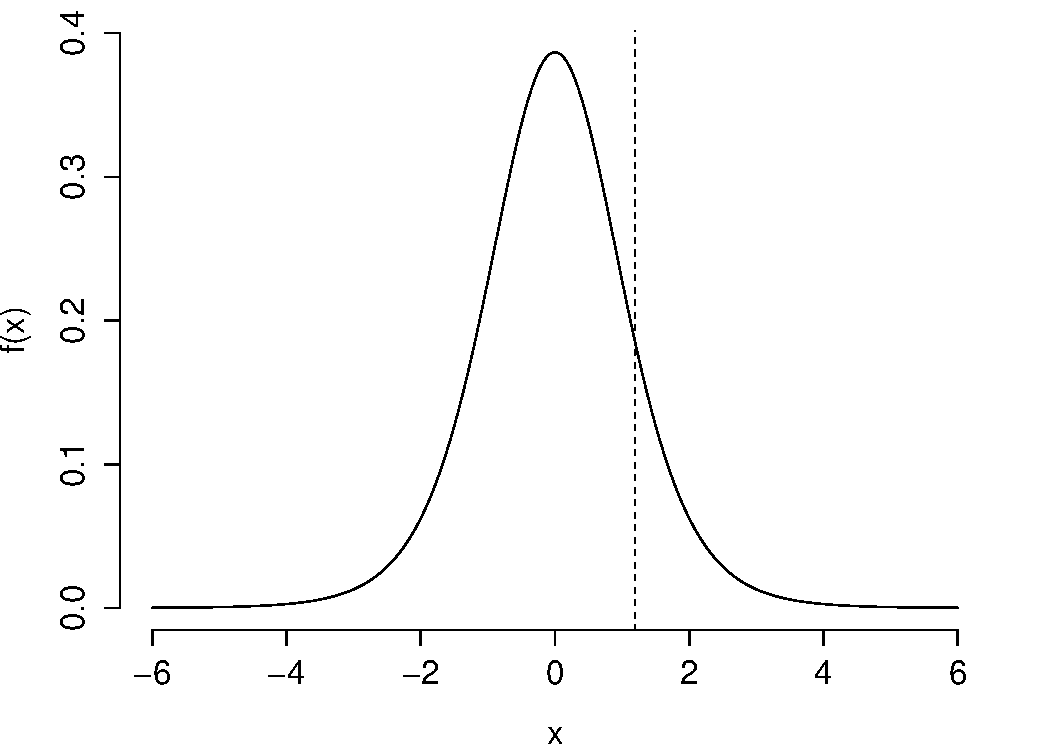
\includegraphics[scale= 0.4]{./images/p_upper2}

\end{figure}

\end{frame}

%%%%%%%%%%%%%%%%%%%%%%%%%%%%%%%%%%%%%%%%
\begin{frame}
\frametitle{What is the p-value? (One-sided Test)}
\footnotesize
Recall: p-value is \emph{smallest significance level} at which our observed test statistic would cause us to reject $H_0$. \alert{Test statistic is $1.14$. What is the one-sided p-value? }
\begin{figure}
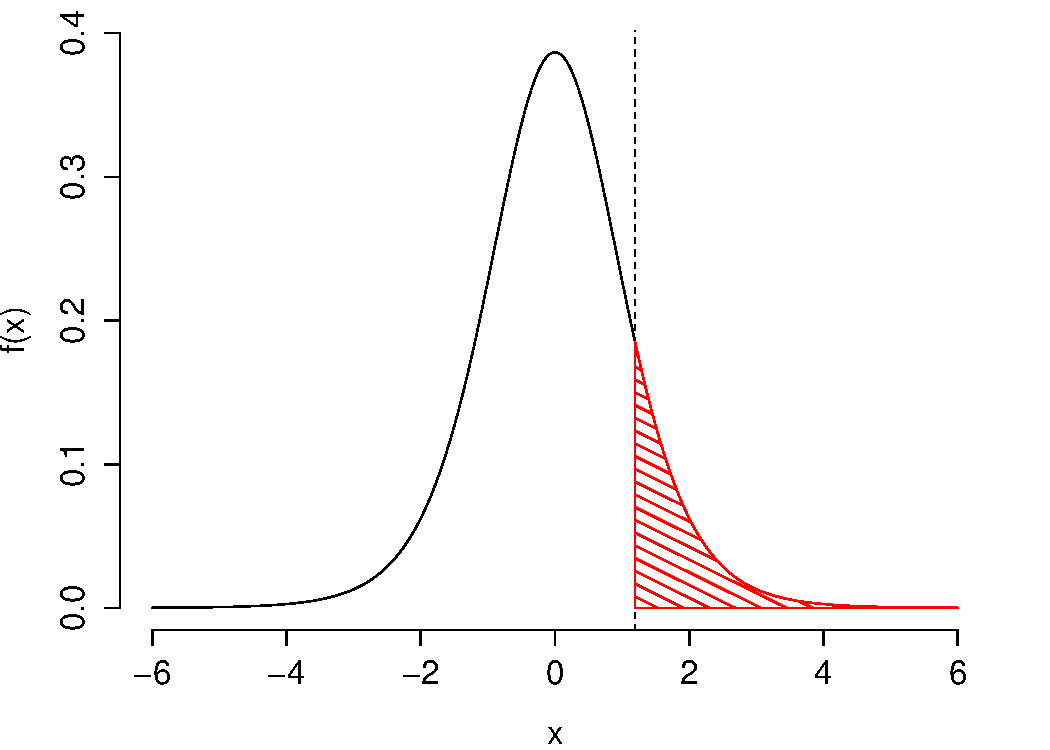
\includegraphics[scale= 0.4]{./images/p_upper3}

\end{figure}

\end{frame}

%%%%%%%%%%%%%%%%%%%%%%%%%%%%%%%%%%%%%%%%
\begin{frame}
\frametitle{What is the p-value? (One-sided Test)}
\footnotesize
Recall: p-value is \emph{smallest significance level} at which our observed test statistic would cause us to reject $H_0$. \alert{Test statistic is $1.14$. What is the one-sided p-value? }
\begin{figure}
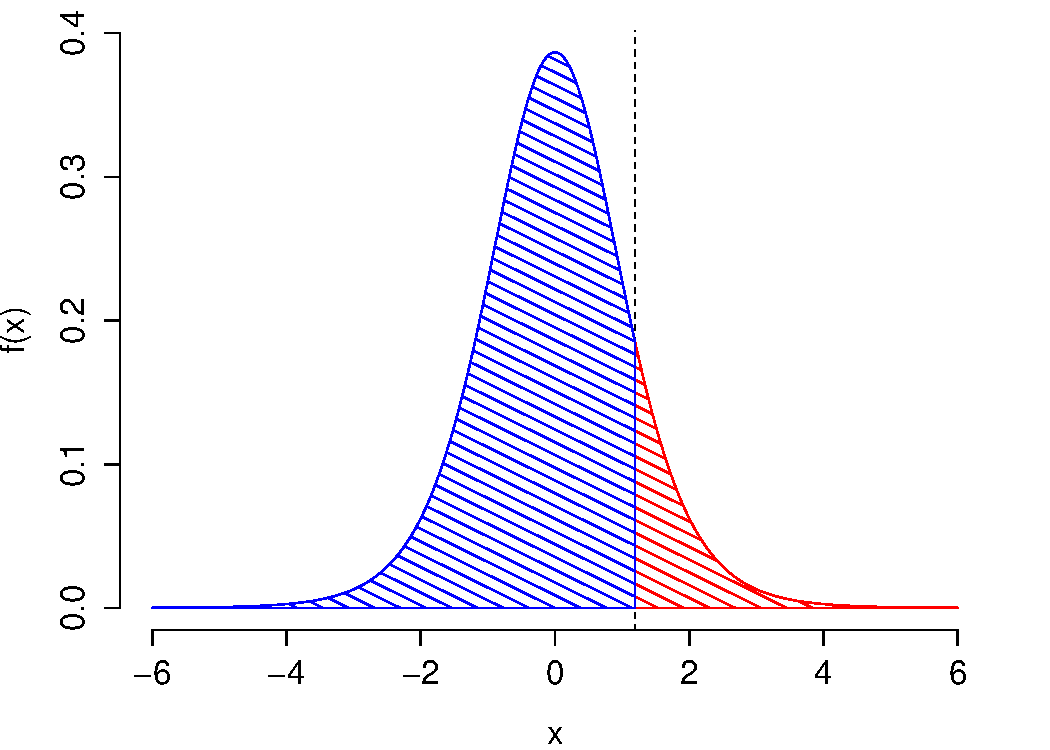
\includegraphics[scale= 0.4]{./images/p_upper4}

\end{figure}

\end{frame}

%%%%%%%%%%%%%%%%%%%%%%%%%%%%%%%%%%%%%%%%
\begin{frame}
\frametitle{What is the p-value? (One-sided Test)}
\footnotesize
Recall: p-value is \emph{smallest significance level} at which our observed test statistic would cause us to reject $H_0$. \alert{Test statistic is $1.14$. What is the one-sided p-value? }
\begin{figure}
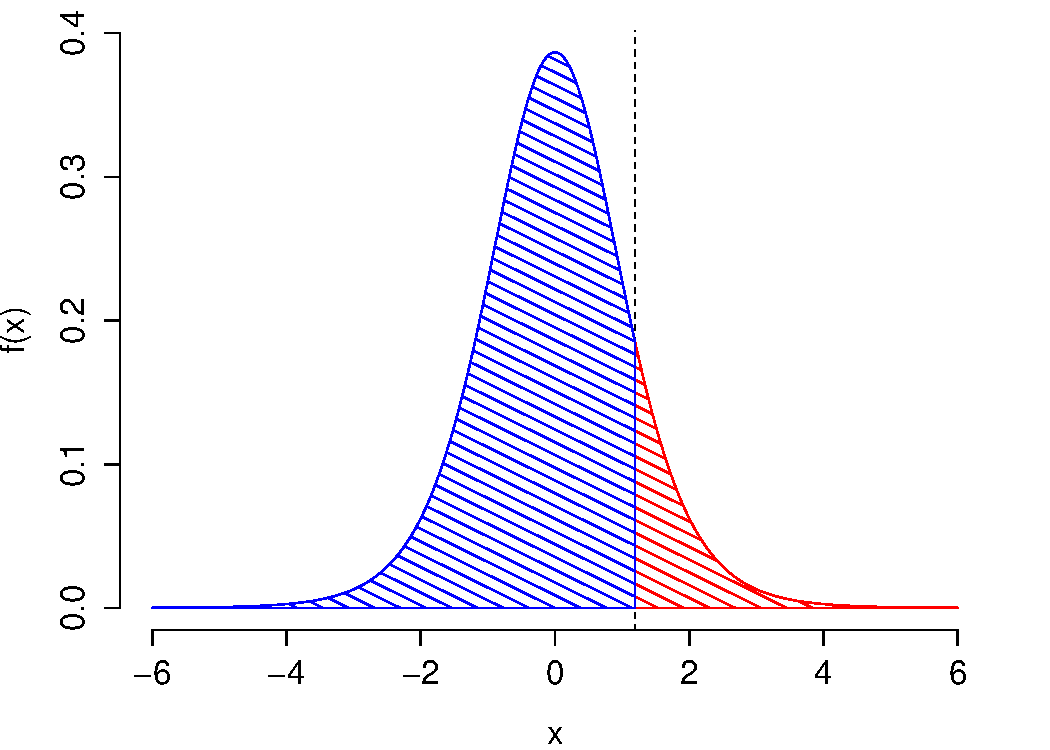
\includegraphics[scale= 0.4]{./images/p_upper4}

\end{figure}
\texttt{1 - pt(1.14, df = 8)}$\approx 0.14$
\end{frame}

%%%%%%%%%%%%%%%%%%%%%%%%%%%%%%%%%%%%%%%%
\begin{frame}
\frametitle{What is the p-value? (Two-sided Test)}
\footnotesize
Recall: p-value is \emph{smallest significance level} at which our observed test statistic would cause us to reject $H_0$. \alert{Test statistic is $1.14$. What is the two-sided p-value? }
\begin{figure}
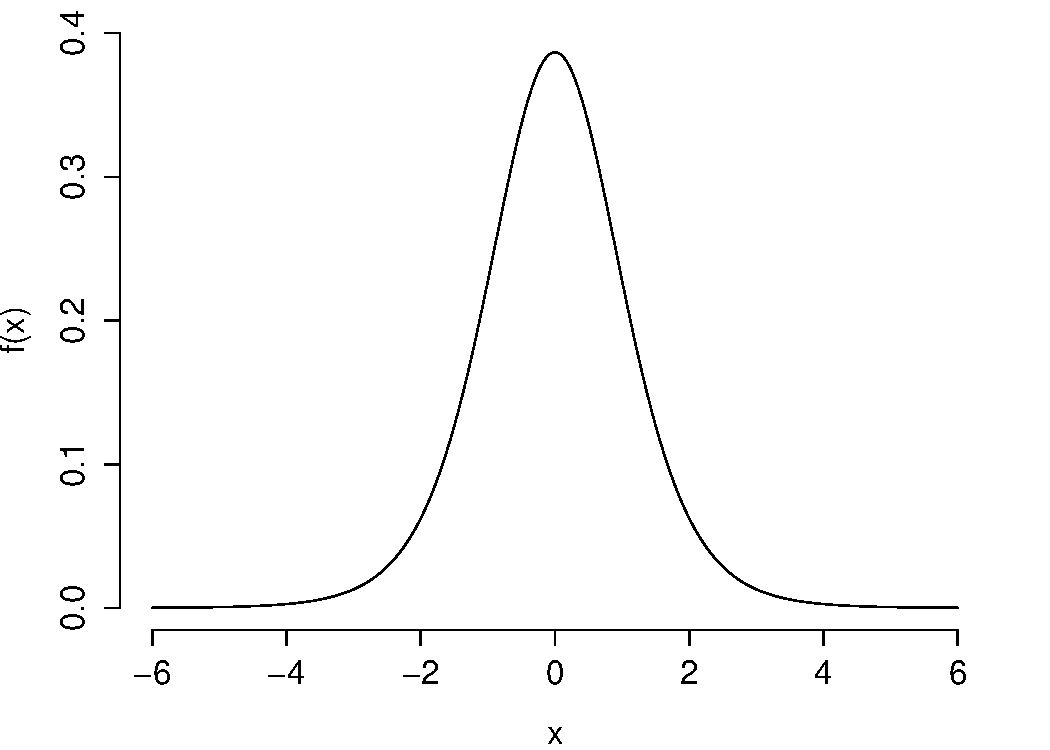
\includegraphics[scale= 0.4]{./images/p_both1}

\end{figure}

\end{frame}

%%%%%%%%%%%%%%%%%%%%%%%%%%%%%%%%%%%%%%%%
\begin{frame}
\frametitle{What is the p-value? (Two-sided Test)}
\footnotesize
Recall: p-value is \emph{smallest significance level} at which our observed test statistic would cause us to reject $H_0$. \alert{Test statistic is $1.14$. What is the two-sided p-value? }
\begin{figure}
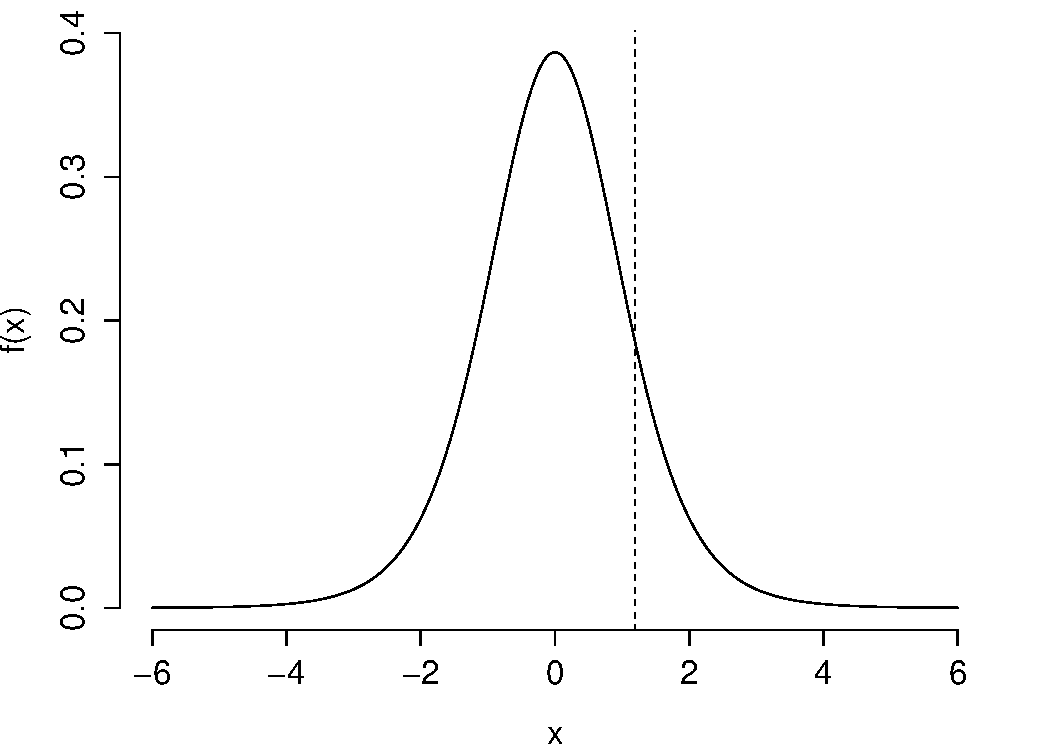
\includegraphics[scale= 0.4]{./images/p_both2}

\end{figure}

\end{frame}

%%%%%%%%%%%%%%%%%%%%%%%%%%%%%%%%%%%%%%%%
\begin{frame}
\frametitle{What is the p-value? (Two-sided Test)}
\footnotesize
Recall: p-value is \emph{smallest significance level} at which our observed test statistic would cause us to reject $H_0$. \alert{Test statistic is $1.14$. What is the two-sided p-value? }
\begin{figure}
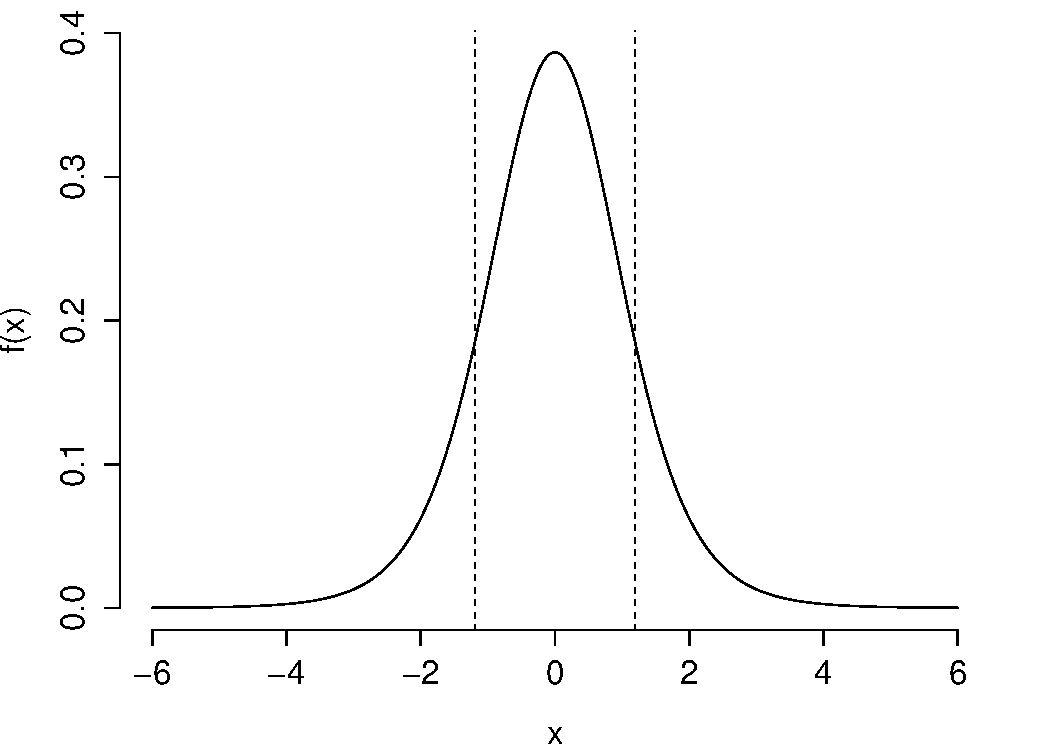
\includegraphics[scale= 0.4]{./images/p_both3}

\end{figure}

\end{frame}

%%%%%%%%%%%%%%%%%%%%%%%%%%%%%%%%%%%%%%%%
\begin{frame}
\frametitle{What is the p-value? (Two-sided Test)}
\footnotesize
Recall: p-value is \emph{smallest significance level} at which our observed test statistic would cause us to reject $H_0$. \alert{Test statistic is $1.14$. What is the two-sided p-value? }
\begin{figure}
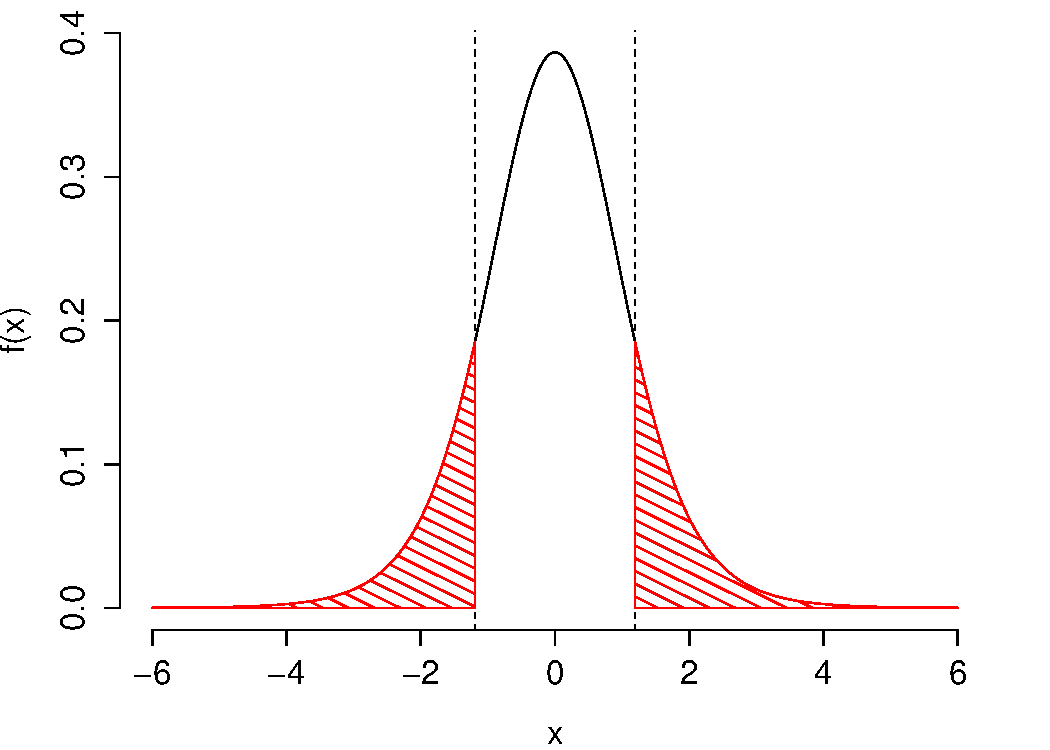
\includegraphics[scale= 0.4]{./images/p_both4}

\end{figure}

\end{frame}

%%%%%%%%%%%%%%%%%%%%%%%%%%%%%%%%%%%%%%%%
\begin{frame}
\frametitle{What is the p-value? (Two-sided Test)}
\footnotesize
Recall: p-value is \emph{smallest significance level} at which our observed test statistic would cause us to reject $H_0$. \alert{Test statistic is $1.14$. What is the two-sided p-value? }
\begin{figure}
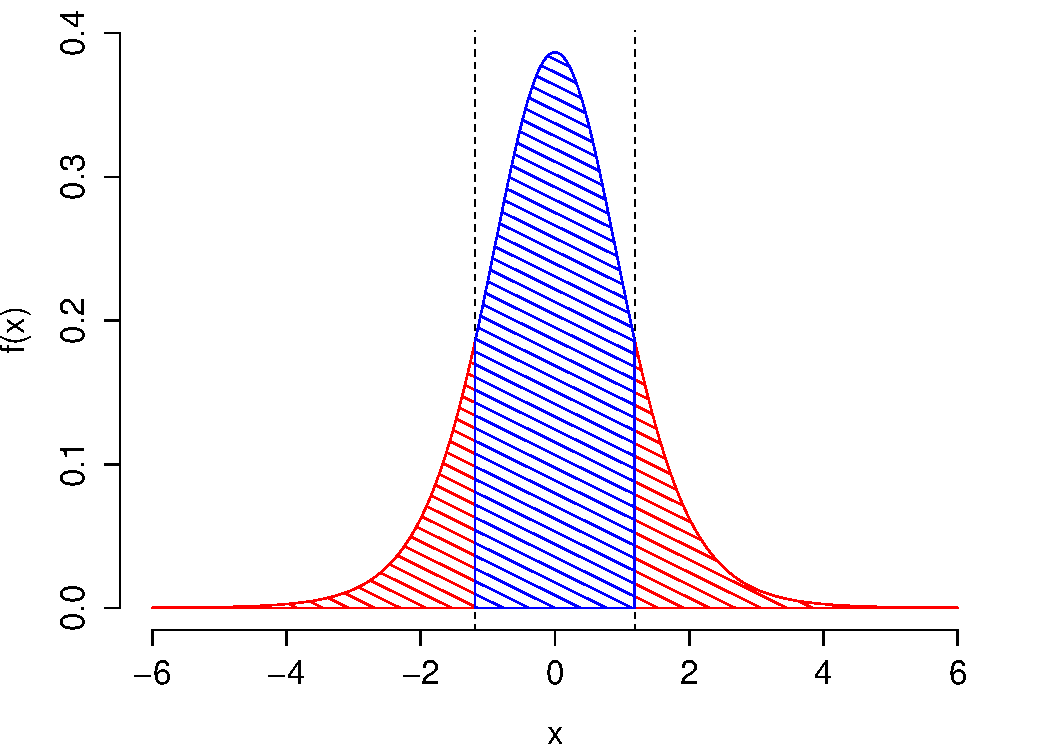
\includegraphics[scale= 0.4]{./images/p_both5}

\end{figure}

\end{frame}

%%%%%%%%%%%%%%%%%%%%%%%%%%%%%%%%%%%%%%%%
\begin{frame}
\frametitle{What is the p-value? (Two-sided Test)}
\footnotesize
Recall: p-value is \emph{smallest significance level} at which our observed test statistic would cause us to reject $H_0$. \alert{Test statistic is $1.14$. What is the two-sided p-value? }
\begin{figure}
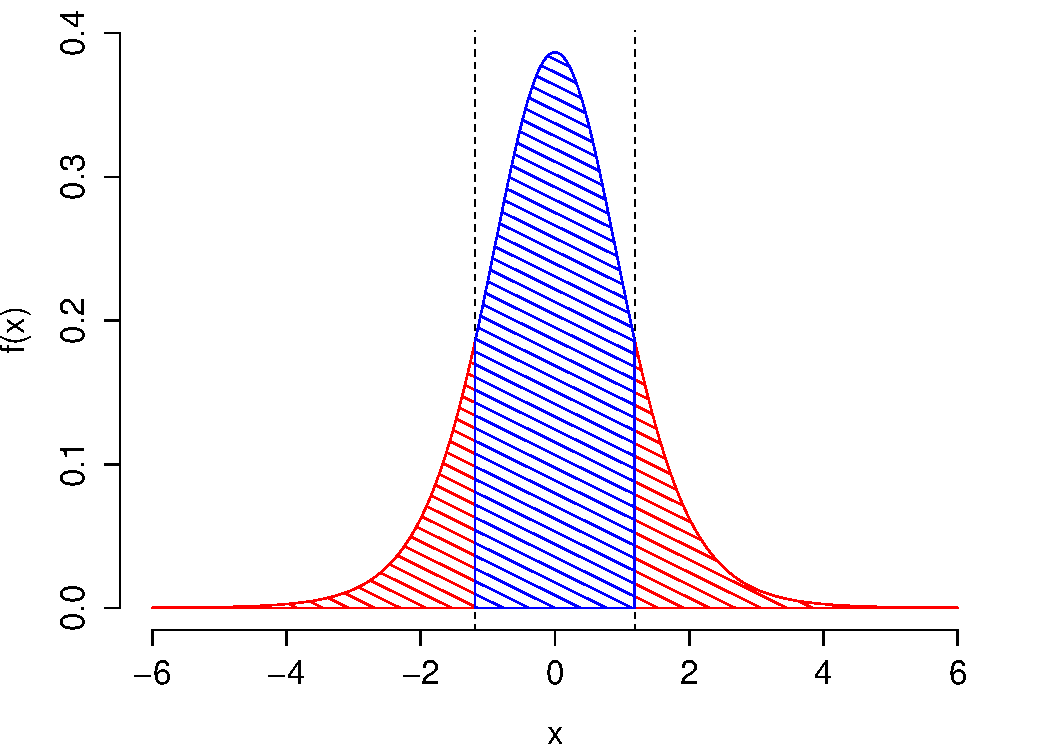
\includegraphics[scale= 0.4]{./images/p_both5}
\end{figure}

\texttt{2 * pt(-1.14, df = 8)}$\approx 0.28$ \pause \hfill \alert{This is twice the one-sided p-value!}
\end{frame}

%%%%%%%%%%%%%%%%%%%%%%%%%%%%%%%%%%%%%%%%

\begin{frame}
\frametitle{Two-sided Test is More Stringent}
\begin{block}{P-value measures strength of evidence against $H_0$}
Lower p-value means stronger evidence. 
\end{block}

\begin{block}{(Two-sided p-value) $= 2 \; \times$  (one-sided p-value)}
Reject $H_0$ based on two-sided test $\implies$ Reject $H_0$ based on appropriate one-sided test. The converse is \emph{false}.
\end{block}


\end{frame}
%%%%%%%%%%%%%%%%%%%%%%%%%%%%%%%%%%%%%%%%

\begin{frame}
\frametitle{Steps in Hypothesis Testing}

\begin{enumerate}
\item Specify Null and Alternative Hypotheses
\item Identify a Test Statistic: a function of the data that has a known sampling distribution under the null.
\item Specify a Decision Rule and a Critical Value so the Type I Error Rate equals $\alpha$.
\end{enumerate}

\begin{alertblock}{Alternative to Step 3}
	Calculate P-Value: the minimum significance level  ($\alpha$) at which we would reject $H_0$ given the observed data.
\end{alertblock}

\end{frame}


%%%%%%%%%%%%%%%%%%%%%%%%%%%%%%%%%%%%%%%%
\begin{frame}
\frametitle{How to Handle Other Examples?}

\alert{You already know lots of sampling distributions! Testing is very similar to constructing confidence intervals in that the steps are always the same, and the only thing that differs is \emph{which} sampling distribution we work with. We'll look at more examples next time.}

\end{frame}
%%%%%%%%%%%%%%%%%%%%%%%%%%%%%%%%%%%%%%%%


%%%%%%%%%%%%%%%%%%%%%%%%%%%%%%%%%%%%%%%%
\begin{frame}
\begin{block}
	{Last Time}
	Walked through steps of hypothesis testing in a simple example.
\end{block}
\begin{alertblock}
	{Today}
	\begin{itemize}
		\item Relationship between hypothesis testing and CIs
		\item More examples of hypothesis tests
	\end{itemize}
\end{alertblock}
\end{frame}


%%%%%%%%%%%%%%%%%%%%%%%%%%%%%%%%%%%%%%%%
\begin{frame}
	\frametitle{Relationship between CI and Two-Sided Test}

	\begin{itemize}
		\item There is a \emph{very close} relationship between CIs and hypothesis tests against a two-sided alternative.
		\item I'll illustrate this using a generic version of the example from last class but the relationship holds \emph{in general}.
	\end{itemize}
\end{frame}
%%%%%%%%%%%%%%%%%%%%%%%%%%%%%%%%%%%%%%%%
\begin{frame}
\frametitle{Relationship between CI and Two-sided Test}
Suppose $X_1, \hdots, X_n \sim \mbox{iid } N(\mu,\sigma^2)$

\vspace{1em}
	\begin{block}{Test $H_0\colon \mu = \mu_0$ vs.\ $H_1\colon \mu \neq \mu_0$ at significance level $\alpha$} 
		\begin{itemize}
			\item Test Statistic:  $T_n = \sqrt{n}(\bar{X}_n - \mu_0)/S \sim t(n-1)$ under $H_0$ 
			\item Decision Rule: Reject $H_0$ if $|T_n| > \texttt{qt}(1-\alpha/2, \texttt{df}=n-1)$ 
			\end{itemize}

			\pause
\end{block}
	\begin{block}{$100\times (1-\alpha)\%$ CI for $\mu$} 
		$$\bar{X}_n \pm \texttt{qt}(1-\alpha/2, \texttt{df}=n-1) \frac{S}{\sqrt{n}}$$
\end{block}
\end{frame}
%%%%%%%%%%%%%%%%%%%%%%%%%%%%%%%%%%%%%%%%
\begin{frame}
\frametitle{Relationship between CI and Two-sided Test}
$\alert{c =  \texttt{qt}(1-\alpha/2, \texttt{df}=n-1)}$
\begin{block}{Decision Rule: Reject $H_0$ if}
		$$\left|\frac{\bar{X}_n - \mu_0}{S/\sqrt{n}} \right|> c \quad \iff \pause  \quad \left(\frac{\bar{X}_n - \mu_0}{S/\sqrt{n}}> c \;\;\mbox{  \alert{OR}  }\;\;\frac{\bar{X}_n - \mu_0}{S/\sqrt{n}}< - c\right)$$
\end{block}

\pause
\begin{block}{Equivalent to: \emph{Don't Reject} $H_0$ provided}
	$$-c \leq \frac{\bar{X}_n - \mu_0}{S/\sqrt{n}}\leq c $$ \pause
	$$\alert{\bar{X_n} - c\times \frac{S}{\sqrt{n}} \leq \mu_0 \leq \bar{X_n} + c\times \frac{S}{\sqrt{n}}}$$
\end{block}
\end{frame}
%%%%%%%%%%%%%%%%%%%%%%%%%%%%%%%%%%%%%%%%
\begin{frame}
\frametitle{What does this mean?}

\begin{block}
	{Two-sided Test $\iff$ Checking if $\mu_0 \in$ CI}
	A two-sided test of $H_0\colon \mu = \mu_0$ against $H_1\colon \mu\neq \mu_0 $ at significance level $\alpha$ is equivalent to checking whether $\mu_0$ lies inside the corresponding $100\times (1-\alpha)\%$ confidence interval for $\mu$.
\end{block}

\pause

\begin{block}
	{``Inverting'' Two-sided Test to get a CI}	
	Collect all the values $\mu_0$ such that we cannot reject $H_0\colon \mu = \mu_0$ against the two-sided alternative. The result is \emph{precisely} a $100\times (1-\alpha)\%$ CI for $\mu$.
\end{block}
\end{frame}
%%%%%%%%%%%%%%%%%%%%%%%%%%%%%%%%%%%%%%%%
%%%%%%%%%%%%%%%%%%%%%%%%%%%%%%%%%%%%%%%%
\begin{frame}
\frametitle{The Anchoring Experiment}
\begin{figure}
\centering
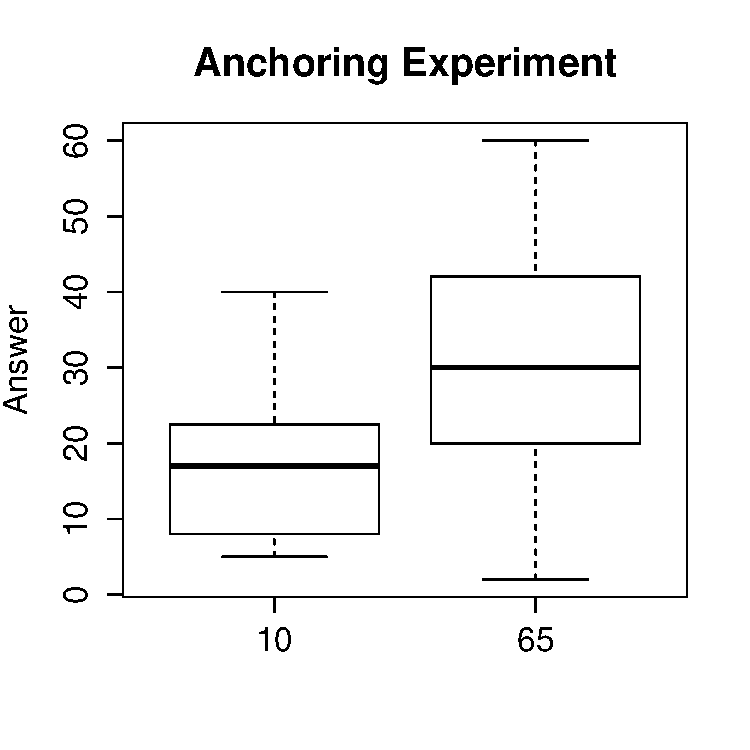
\includegraphics[scale = 0.55]{./images/anchoring_boxplot}
\end{figure}
\end{frame}
%%%%%%%%%%%%%%%%%%%%%%%%%%%%%%%%%%%%%%%%%
\begin{frame}
\frametitle{The Anchoring Experiment}
Shown a ``random'' number and then asked what proportion of UN member states are located in Africa.
	\begin{block}{``Hi'' Group -- Shown 65 ($n_{Hi}=46$)}
		Sample Mean: $30.7$, Sample Variance: $253$
\end{block}


	\begin{block}{``Lo'' Group -- Shown 10 ($n_{Lo}=43$)}
	Sample Mean: $17.1$, Sample Variance: $86$
\end{block}


\vspace{1em}

\hfill\alert{\fbox{Fairly large samples here, so we'll proceed via the CLT...}}
\end{frame}
%%%%%%%%%%%%%%%%%%%%%%%%%%%%%%%%%%%%%%%

\begin{frame}
	\frametitle{In words, what is our null hypothesis?\hfill 
\includegraphics[scale = 0.05]{./images/clicker}}

	\begin{enumerate}[(a)]
		\item There is a \emph{positive} anchoring effect: seeing a higher random number makes people report a higher answer.
		\item There is a \emph{negative} anchoring effect: seeing a lower random number makes people report a lower answer. 
		\item There \emph{is} an anchoring effect: it could be positive or negative.
		\item There is  \emph{no} anchoring effect: people aren't influenced by seeing a random number before answering.
	\end{enumerate}
\end{frame}
%%%%%%%%%%%%%%%%%%%%%%%%%%%%%%%%%%%%%%%
\begin{frame}
	\frametitle{In symbols, what is our null hypothesis?\hfill 
\includegraphics[scale = 0.05]{./images/clicker}}

	\begin{enumerate}[(a)]
		\item $\mu_{Lo} < \mu_{Hi}$
		\item $\mu_{Lo} = \mu_{Hi}$
		\item $\mu_{Lo} > \mu_{Hi}$
		\item $\mu_{Lo} \neq \mu_{Hi}$
	\end{enumerate}
\pause
	\vspace{1em}

	\alert{$\mu_{Lo} = \mu_{Hi}$ is \emph{equivalent to} $\mu_{Hi} - \mu_{Lo} = 0$!}
\end{frame}
%%%%%%%%%%%%%%%%%%%%%%%%%%%%%%%%%%%%%%%
\begin{frame}
	\frametitle{Anchoring Experiment\hfill 
\includegraphics[scale = 0.05]{./images/clicker}}
 
Under the null, what should we expect to be true about the values taken on by $\bar{X}_{Lo}$ and $\bar{X}_{Hi}$?

\vspace{1em}

	\begin{enumerate}[(a)]
		\item They should be similar in value.
		\item $\bar{X}_{Lo}$ should be the smaller of the two.
		\item $\bar{X}_{Hi}$ should be the smaller of the two.
		\item They should be different. We don't know which will be larger.
	\end{enumerate}
\end{frame}
%%%%%%%%%%%%%%%%%%%%%%%%%%%%%%%%%%%%%%%%

\begin{frame}
\frametitle{What is our Test Statistic?}
\begin{block}{Sampling Distribution}
		$$\frac{\left(\bar{X}_{Hi} - \bar{X}_{Lo}\right) - \left(\mu_{Hi} - \mu_{Lo}\right)}{\sqrt{\frac{S_{Hi}^2}{n_{Hi}} + \frac{S_{Lo}^2}{n_{Lo}}}} \approx N(0,1)$$
\end{block}

\begin{block}{Test Statistic: Impose the Null}
Under $H_0\colon \mu_{Lo} = \mu_{Hi}$
	$$T_n =\frac{\bar{X}_{Hi} - \bar{X}_{Lo}}{\sqrt{\frac{S_{Hi}^2}{n_{Hi}} + \frac{S_{Lo}^2}{n_{Lo}}}} \approx N(0,1)$$
\end{block}
\end{frame}


%%%%%%%%%%%%%%%%%%%%%%%%%%%%%%%%%%%%%%%%
\begin{frame}
\frametitle{What is our Test Statistic?}
\footnotesize
$\bar{X}_{Hi} = 30.7$, $s^2_{Hi} = 253$, $n_{Hi} = 46$\\
$\bar{X}_{Lo} = 17.1$, $s^2_{Lo} = 86$, $n_{Lo} = 43$\\
\normalsize
\vspace{2em}

\begin{block}{Under $H_0\colon \mu_{Lo} = \mu_{Hi}$}
	$$T_n = \frac{\bar{X}_{Hi} - \bar{X}_{Lo}}{\sqrt{\frac{S_{Hi}^2}{n_{Hi}} + \frac{S_{Lo}^2}{n_{Lo}}}} \approx N(0,1)$$
\end{block}

\begin{block}{Plugging in Our Data}
$$T_n = \frac{\bar{X}_{Hi} - \bar{X}_{Lo}}{\sqrt{\frac{S_{Hi}^2}{n_{Hi}} + \frac{S_{Lo}^2}{n_{Lo}}}} \approx 5$$
\end{block}
\end{frame}


%%%%%%%%%%%%%%%%%%%%%%%%%%%%%%%%%%%%%%%%
\begin{frame}[t]
\frametitle{Anchoring Experiment Example \hfill 
\includegraphics[scale = 0.05]{./images/clicker}}
Approximately what critical value should we use to test $H_0\colon \mu_{Lo} = \mu_{Hi}$ against the two-sided alternative at the 5\% significance level?

\pause
\vspace{1em}
\begin{center}
\begin{tabular}{l|lll}
$\alpha$ &   0.10& 0.05 &0.01\\
\hline
\texttt{qnorm($1-\alpha$)} & 1.28 &1.64 &2.33\\
\texttt{qnorm($1-\alpha/2$)} &1.64 &\alert{1.96}& 2.58
\end{tabular}
\end{center}
\hfill \alert{... Approximately 2}
\end{frame}
%%%%%%%%%%%%%%%%%%%%%%%%%%%%%%%%%%%%%%%%
\begin{frame}
\frametitle{Anchoring Experiment Example\hfill 
\includegraphics[scale = 0.05]{./images/clicker}}
Which of these commands would give us the p-value of our test of $H_0\colon \mu_{Lo} = \mu_{Hi}$ against $H_1\colon \mu_{Lo}<\mu_{Hi}$ at significance level $\alpha$?
\vspace{1em}
	\begin{enumerate}[(a)]
		\item \texttt{qnorm($1-\alpha$)}
		\item \texttt{qnorm($1-\alpha/2$)}
		\item \texttt{1 - pnorm(5)}
		\item \texttt{2 * (1 - pnorm(5))}
	\end{enumerate}
	

\end{frame}
%%%%%%%%%%%%%%%%%%%%%%%%%%%%%%%%%%%%%%%%

\begin{frame}
\frametitle{P-values for $H_0\colon \mu_{Lo} = \mu_{Hi}$}
We plug in the value of the test statistic that we observed: 5
\begin{block}{Against $H_1\colon \mu_{Lo}< \mu_{Hi}$}
\texttt{1 - pnorm(5)} $< 0.0000$
\end{block}

\begin{block}{Against $H_1\colon \mu_{Lo}\neq \mu_{Hi}$}
\texttt{2 * (1 - pnorm(5))} $< 0.0000$
\end{block}

\vspace{1em}

\alert{If the null is true (the two population means are equal) it would be extremely unlikely to observe a test statistic as large as this!}

\vspace{1em} 
\hfill \fbox{What should we conclude?}
\end{frame}


%%%%%%%%%%%%%%%%%%%%%%%%%%%%%%%%%%%%%%%%
\begin{frame}
\frametitle{Which Exam is Harder?}
% latex.default(round(grades.out, 1), file = "grades.tex", rowname = NULL) 
%
\begin{table}[!tbp]
\begin{center}
\begin{tabular}{rccr}
\hline\hline
\multicolumn{1}{r}{Student}&\multicolumn{1}{c}{Exam 1}&\multicolumn{1}{c}{Exam 2}&\multicolumn{1}{r}{Difference}\tabularnewline
\hline
$ 1$&$57.1$&$60.7$&$  3.6$\tabularnewline
\vdots&\vdots&\vdots&\vdots\\
$71$&$78.6$&$82.9$&$  4.3$\tabularnewline
\hline
Sample Mean: & 79.6 & 81.4  &1.8\\
Sample Var. &117  & 151 & 124\\
Sample Corr.& \multicolumn{2}{c}{0.54}&\\
\hline
\end{tabular}
\end{center}
\end{table}

\vspace{1em}

\fbox{Again, large sample size here so we'll use CLT.}
\end{frame}
%%%%%%%%%%%%%%%%%%%%%%%%%%%%%%%%%%%%%%%%
\begin{frame}
\frametitle{One-Sample Hypothesis Test Using Differences}
\small
\fbox{Let $D_i = X_i - Y_i$ be (Midterm 2 Score - Midterm 1 Score) for student $i$}
\vspace{0.1em}
\begin{block}{Null Hypothesis}
$H_0\colon \mu_1 = \mu_2$, i.e.\ both exams were of the same difficulty
\end{block}
\begin{block}{Two-Sided Alternative}
$H_1\colon \mu_1 \neq \mu_2$, i.e.\ one exam was harder than the other
\end{block}
\begin{block}{One-Sided Alternative}
$H_1\colon \mu_2 > \mu_1$, i.e.\ the second exam was easier
\end{block}
\end{frame}
%%%%%%%%%%%%%%%%%%%%%%%%%%%%%%%%%%%%%%%%

\begin{frame}
\frametitle{Decision Rules}
\small
\fbox{Let $D_i = X_i - Y_i$ be (Midterm 2 Score - Midterm 1 Score) for student $i$}
\vspace{0.1em}


\begin{block}
	{Test Statistic}
$$\displaystyle \frac{\bar{D}_n}{\widehat{SE}(\bar{D}_n)}=\frac{1.8}{\sqrt{124/71}} \approx 1.36$$
\end{block}


\begin{block}{Two-Sided Alternative} 
Reject $H_0\colon \mu_1 = \mu_2$ in favor of $H_1\colon \mu_1 \neq \mu_2$ if $|\bar{D}_n|$ is sufficiently large.
\end{block}
\begin{block}{One-Sided Alternative}
Reject $H_0\colon \mu_1 = \mu_2$ in favor of $H_1\colon \mu_2 >\mu_1$ if $\bar{D}_n$ is sufficiently large.
\end{block}
\end{frame}
%%%%%%%%%%%%%%%%%%%%%%%%%%%%%%%%%%%%%%%%

\begin{frame}
\frametitle{Reject against \emph{Two-sided} Alternative with $\alpha = 0.1$?  
\includegraphics[scale = 0.05]{./images/clicker}}

	$$\boxed{\displaystyle \frac{\bar{D}_n}{\widehat{SE}(\bar{D}_n)}= \frac{1.8}{\sqrt{124/71}} \approx 1.36} $$

\begin{center}
\begin{tabular}{l|lll}
$\alpha$ &   0.10& 0.05 &0.01\\
\hline
\texttt{qnorm($1-\alpha$)} & 1.28 &1.64 &2.33\\
\texttt{qnorm($1-\alpha/2$)} &1.64 &1.96& 2.58
\end{tabular}
\end{center}

\begin{enumerate}[(a)]
\item Reject
\item Fail to Reject
\item Not Sure
\end{enumerate}

\end{frame}

%%%%%%%%%%%%%%%%%%%%%%%%%%%%%%%%%%%%%%%%
\begin{frame}
\frametitle{Reject against \emph{One-sided} Alternative with $\alpha = 0.1$?  
\includegraphics[scale = 0.05]{./images/clicker}}

	$$\boxed{\displaystyle \frac{\bar{D}_n}{\widehat{SE}(\bar{D}_n)}= \frac{1.8}{\sqrt{124/71}} \approx 1.36} $$

\begin{center}
\begin{tabular}{l|lll}
$\alpha$ &   0.10& 0.05 &0.01\\
\hline
\texttt{qnorm($1-\alpha$)} & 1.28 &1.64 &2.33\\
\texttt{qnorm($1-\alpha/2$)} &1.64 &1.96& 2.58
\end{tabular}
\end{center}

\begin{enumerate}[(a)]
\item Reject
\item Fail to Reject
\item Not Sure
\end{enumerate}



\end{frame}

%%%%%%%%%%%%%%%%%%%%%%%%%%%%%%%%%%%%%%%%
\begin{frame}
\frametitle{P-Values for the Test of $H_0\colon \mu_1 = \mu_2$}

	$$\boxed{\displaystyle \frac{\bar{D}_n}{\widehat{SE}(\bar{D}_n)}= \frac{1.8}{\sqrt{124/71}} \approx 1.36} $$

\begin{block}{One-Sided $H_1\colon \mu_2 > \mu_1 $} 
$\texttt{1 - pnorm(1.36)} =  \texttt{pnorm(-1.36)}  \approx 0.09$ 
\end{block}

\begin{block}{Two-Sided $H_1 \colon \mu_1 \neq \mu_2$} 
$\texttt{2 * (1 - pnorm(1.36))} =  \texttt{2 * pnorm(-1.36)} \approx 0.18$
\end{block}
\end{frame}
%%%%%%%%%%%%%%%%%%%%%%%%%%%%%%%%%%%%%%%%
\begin{frame}
	\frametitle{Tests for Proportions}
	\begin{block}
		{Basic Idea}
		The population \emph{can't be} normal (it's Bernoulli) so we use the CLT to get approximate sampling distributions (c.f.\ Lecture 18).
	\end{block}
	\begin{block}
		{But there's a small twist!}
		Bernoulli RV only has a \emph{single} unknown parameter $\implies$  we know \emph{more} about the population under $H_0$ in a proportions problem than in the other testing examples we've examined...	
	\end{block}

\vspace{1em}	

	\hfill\alert{\fbox{For best results, always \emph{fully} impose the null.}}
\end{frame}

%%%%%%%%%%%%%%%%%%%%%%%%%%%%%%%%%%%%%%%%
\begin{frame}
	\frametitle{Tests for Proportions: One-Sample Example}
	\begin{block}
		{From Pew Polling Data}
		54\% of a random sample of 771 registered voters correctly identified 2012 presidential candidate Mitt Romney as Pro-Life.
	\end{block}
	\begin{block}
		{Sampling Model}
		$X_1, \hdots, X_{n} \sim \mbox{iid Bernoulli}(p)$
	\end{block}
	\begin{block}
		{Sample Statistic}
		Sample Proportion: $\displaystyle\widehat{p} = \frac{1}{n}\sum_{i=1}^{n} X_i$
	\end{block}

	\vspace{1em}

	\hfill \alert{\fbox{Suppose I wanted to test $H_0\colon p = 0.5$}}
\end{frame}
%%%%%%%%%%%%%%%%%%%%%%%%%%%%%%%%%%%%%%%%
\begin{frame}
	\frametitle{Tests for Proportions: One Sample Example}
	Under $H_0\colon p = 0.5$ what is the standard error of $\widehat{p}$?

	\begin{enumerate}[(a)]
		\item $1$
		\item $\sqrt{\widehat{p}(1-\widehat{p})/n}$
		\item $\sigma/\sqrt{n}$
		\item $1/(2\sqrt{n})$
		\item $p(1-p)$ 
	\end{enumerate}
\pause
 \alert{$p=0.5 \implies \sqrt{0.5(1-0.5)/n} = 1/(2\sqrt{n})$}

 \vspace{1em}
 \emph{Under the null we know the SE! Don't have to estimate it!}

\end{frame}
%%%%%%%%%%%%%%%%%%%%%%%%%%%%%%%%%%%%%%%%
\begin{frame}
	\frametitle{One-Sample Test for a Population Proportion}
	\begin{block}
		{Sampling Model}
		$X_1, \hdots, X_n \sim \mbox{iid Bernoulli}(p)$
	\end{block}
	\begin{block}
		{Null Hypothesis}
		$H_0 \colon p = \mbox{Known Constant } p_0$
	\end{block}
	\begin{block}
		{Test Statistic} 
		$\displaystyle T_n = \frac{\widehat{p} - p_0}{\sqrt{p_0(1-p_0)/n}} \approx N(0,1)$ under $H_0$ provided $n$ is large
	\end{block}
\end{frame}
%%%%%%%%%%%%%%%%%%%%%%%%%%%%%%%%%%%%%%%%
\begin{frame}
	\frametitle{One-Sample Example $H_0\colon p = 0.5$}
	\fbox{\footnotesize 54\% of a random sample of 771 registered voters knew Mitt Romney is Pro-Life.}

\vspace{1em}

	\begin{eqnarray*}
		T_n &=& \frac{\widehat{p} - p_0}{\sqrt{\displaystyle \frac{p_0(1 - p_0)}{n}}} = 2 \sqrt{771}(0.54 - 0.5)\\ \\
		&=& 0.08 \times \sqrt{771} \approx 2.2
	\end{eqnarray*}
	\begin{block}
		{One-Sided p-value}
		\texttt{1 - pnorm(2.2)} $\approx 0.014$
	\end{block}
	\begin{block}
		{Two-Sided p-value}
		\texttt{2 * (1 - pnorm(2.2))} $\approx 0.028$
	\end{block}
\end{frame}
%%%%%%%%%%%%%%%%%%%%%%%%%%%%%%%%%%%%%%%%
\begin{frame}
	\frametitle{Tests for Proportions: Two-Sample Example}
	\begin{block}
		{From Pew Polling Data}
		53\% of a random sample of 238 Democrats correctly identified Mitt Romney as Pro-Life versus 61\% of 239 Republicans.
	\end{block}
	\begin{block}
		{Sampling Model}
		Republicans: $X_1, \hdots, X_{n} \sim \mbox{iid Bernoulli}(p)$ independent of\\
		Democrats: $Y_1, \hdots,Y_{m} \sim \mbox{iid Bernoulli}(q)$ 
	\end{block}
	\begin{block}
		{Sample Statistics}
		Sample Proportions: $\displaystyle\widehat{p} = \frac{1}{n}\sum_{i=1}^{n} X_i, \quad\displaystyle\widehat{q} = \frac{1}{m}\sum_{i=1}^{m} Y_i$
	\end{block}

	\vspace{1em}

	\hfill \alert{\fbox{Suppose I wanted to test $H_0\colon p = q$}}
\end{frame}
%%%%%%%%%%%%%%%%%%%%%%%%%%%%%%%%%%%%%%%%
\begin{frame}
	\frametitle{A More Efficient Estimator of the SE Under $H_0$}
	\begin{alertblock}
		{Don't Forget!}
		Standard Error (SE) means ``std.\ dev.\ of sampling distribution'' so you should know how to prove that that:
	$$SE(\widehat{p} - \widehat{q}) = \sqrt{\frac{p(1-p)}{n} + \frac{q(1-q)}{m}}$$
	\end{alertblock}

	\begin{block}
		{Under $H_0\colon p = q$}
		\emph{Don't} know values of $p$ and $q$: only that they are equal.
	\end{block}

\end{frame}
%%%%%%%%%%%%%%%%%%%%%%%%%%%%%%%%%%%%%%%%
\begin{frame}
	\frametitle{A More Efficient Estimator of the SE Under $H_0$}
	\begin{block}
		{One Possible Estimate}
	$$\widehat{SE} = \sqrt{\frac{\widehat{p}(1-\widehat{p})}{n} + \frac{\widehat{q}(1-\widehat{q})}{m}}$$
	\end{block}
	\begin{block}
		{A \emph{Better} Estimate Under $H_0$}
		$$\widehat{SE}_{Pooled} = \sqrt{\widehat{\pi}(1-\widehat{\pi})\left( \frac{1}{n} + \frac{1}{m} \right) } \quad \mbox{where}\quad \widehat{\pi} = \displaystyle \frac{n \widehat{p} + m \widehat{q}}{n + m}$$
	\end{block}
	\begin{alertblock}
		{Why Pool?}
		If $p = q$, the two populations \emph{are the same}. This means we can get a \emph{more precise} estimate of the \emph{common} population proportion by pooling. More data = Lower Variance $\implies$ better estimated SE.
	\end{alertblock}
\end{frame}
%%%%%%%%%%%%%%%%%%%%%%%%%%%%%%%%%%%%%%%%
\begin{frame}
	\frametitle{Two-Sample Test for Proportions}
	\begin{block}
		{Sampling Model}
		\small
		$X_1, \hdots, X_n \sim \mbox{iid Bernoulli}(p)$ indep.\  of $Y_1, \hdots, Y_m \sim \mbox{iid Bernoulli}(q)$
	\end{block}
	\begin{block}
		{Sample Statistics}
			Sample Proportions: $\displaystyle\widehat{p} = \frac{1}{n}\sum_{i=1}^{n} X_i, \quad\displaystyle\widehat{q} = \frac{1}{m}\sum_{i=1}^{m} Y_i$
	\end{block}
	\begin{block}
		{Null Hypothesis}
		$H_0\colon p = q \quad \Leftarrow \; $\fbox{ i.e.\ $p - q = 0$}
	\end{block}
	\begin{block}
		{Pooled Estimator of SE under $H_0$}
		$\widehat{\pi} = \displaystyle \frac{n \widehat{p} + m \widehat{q}}{n + m}, \quad \widehat{SE}_{Pooled} = \sqrt{\widehat{\pi}(1-\widehat{\pi})\left( 1/n + 1/m \right) }$
	\end{block}
	\begin{block}
		{Test Statistic}
		$\displaystyle T_n = \frac{\widehat{p}- \widehat{q}}{\widehat{SE}_{Pooled}} \approx N(0,1)$ under $H_0$ provided $n$ and $m$ are large
	\end{block}
\end{frame}
%%%%%%%%%%%%%%%%%%%%%%%%%%%%%%%%%%%%%%%%
\begin{frame}
	\frametitle{Two-Sample Example $H_0\colon p = q$}
	\fbox{\footnotesize 53\% of 238 Democrats knew Romney is Pro-Life vs.\ 61\% of 239 Republicans}
	\small
$$\widehat{\pi} = \frac{n\widehat{p}+ m\widehat{q}}{n + m} = \frac{239 \times 0.61 + 238 \times 0.53}{239 + 238}\approx 0.57$$
	\begin{eqnarray*}
	\widehat{SE}_{Pooled} &=&  \sqrt{\widehat{\pi}(1-\widehat{\pi})\left( 1/n + 1/m \right) }= \sqrt{0.57 \times 0.43 (1/239 + 1/238)}\\
		&\approx& 0.045
	\end{eqnarray*}
$$T_n = \frac{\widehat{p} - \widehat{q}}{\widehat{SE}_{Pooled}}= \frac{0.61 - 0.53}{0.045} \approx 1.78$$
\begin{block}
	{One-Sided P-Value}
	\texttt{1 - pnorm(1.78)}$\approx 0.04$
\end{block}\begin{block}
	{Two-Sided P-Value}
	\texttt{2 * (1 - pnorm(1.78))}$\approx 0.08$
\end{block}
\end{frame}
%%%%%%%%%%%%%%%%%%%%%%%%%%%%%%%%%%%%%%%%
